

\section{Operational Challenges in Multi-tenant Clusters for Big Data
  Analytics}
\label{sec:sec2}

Managed by a small cluster operations team, Rocket Fuel's multi-tenant Hadoop cluster has approximately 1000 nodes storing over 30 petabytes of data. 
The cluster
supports applications created by many teams within the company.
The operations team has created six pools to manage
multi-tenancy. We will call these pools ETL1, ETL2, APP1, APP2, 
BI, and Default. 

\squishlist
\item The ETL1 pool runs a very large number of jobs every day---many of
which are low-level MapReduce jobs---that perform 
data copying and extract-transform-load (ETL) operations.
\item The ETL2 pool contains a mixed workload that includes advanced SQL
analytics, machine-learning computations, ad-hoc queries, and 
repeated workflows. 
\item The APP pools contain ad-hoc or repeated applications
from different teams. 
\item The BI pool contains ad-hoc queries in SQL with considerable 
use of user-defined functions. 
\item The Default pool is for applications that are not mapped
to one of the other pools. 
\squishend

\vspace{1mm}
\noindent Assignment of applications to these pools 
is done statically. Resources are partitioned dynamically 
among the pools based on the fair share resource allocation 
policy as implemented by Hadoop's {\em Fair} 
scheduler \cite{fair-share-scheduler}. 
 As we will discuss later, how resources are partitioned across pools 
and within a pool are based on configurations defined statically 
by the operations team.

Broadly speaking, the objective of the cluster operations team 
is to maximize cluster performance while meeting the business 
service-level agreements (SLAs). 
However, as part of the overall multi-tenant resource management process, 
the cluster operations team has to serve several, potentially
conflicting, interests. For example, users such as business 
analysts (who use the BI pool) wish to minimize the
latency of their jobs; and show little interest in the overall
performance of the cluster. The manager of a team that is 
responsible for a repeated workflow (e.g., one that 
refreshes a base table used by many time-sensitive analysis tasks)
will only care about ensuring that this workflow gets 
enough resources to finish in time. This workflow may be part
of a number of applications that share the ETL2 pool. 

Multi-tenant scenarios like what we see at Rocket Fuel are now 
common in companies that process large amounts of data. 
The larger heterogeneity (recall Section \ref{sec:intro})
and the more democratic nature of Hadoop usage bring 
unprecedented operational challenges compared to managing 
multi-tenancy in traditional parallel database systems.
In the rest of this section, we aim to create a deeper understanding of 
the problems in multi-tenant resource management. We will use real examples 
of problems seen at Rocket Fuel. In particular, we will look at 
these problems from the perspective of Alice. Alice  is 
a fictional member of the cluster operations team who is
responsible for managing multi-tenancy in the cluster. 

\subsection {Understanding Effective Cluster Utilization}
\label{sec:effective-utilization}

Figures \ref{fig:demand}(a) and \ref{fig:demand}(b)
show graphs that Alice looks at routinely
in order to understand the overall demand for resources 
on the cluster. In Hadoop, the resources in the 
cluster are discretized linearly into {\em slots}. The cluster
contains a total {\em MAP\_SLOTS} number of {\em map slots} and 
{\em REDUCE\_SLOTS}  number of {\em reduce slots}. A map (reduce) 
slot can run one map (reduce) attempt at any point of time.

Figure \ref{fig:demand}(a) (Figure \ref{fig:demand}(b))
plots the {\em demand} for map (reduce) slots
in comparison to the total number of map (reduce) slots available. 
This data is for the time from July 5 to August 4, 2014. 
The map (reduce) demand at a time $t$ is defined as the number of map 
(reduce) attempts that are running or ready to run
at time $t$; also called the number of {\em runnable} map (reduce) 
attempts. A runnable map (reduce) attempt will actually run only when it is 
assigned a map (reduce) slot. The number of runnable attempts 
for a logical map or reduce {\em task} can be greater than one if 
{\em speculative execution} is enabled. In this case, Hadoop will 
identify {\em straggler} attempts for a task that are running more
slowly compared to 
other attempts from the same job; and create additional attempts 
that can be run to complete the task.

Alice can see from Figures \ref{fig:demand}(a) and 
\ref{fig:demand}(b) that, at most points of time, the demand 
for slots far exceeds the total number of available slots. 
This observation means that the multi-tenant cluster is 
almost always under contention, so proper management
of resources is essential. The first question that Alice 
usually has is whether the slots available in the cluster are 
all being used as much as possible. 

Figure \ref{fig:demand}(c) plots the actual {\em usage} of
map (reduce) slots for the same time period from July 5 to August 
4, 2014. Map slot usage $U_m(t)$ is defined  at a time $t$ as follows:
\[
U_{m}(t)=\min\left\{S_{m}(t)-C_{m}(t),\mbox{\em MAP\_SLOTS}\right\}
\]
Here, $S_m(t)$ and $C_m(t)$ denote the number of runnable 
map attemts and completed map attempts, respectively, at
time t. Similarly, $U_r(t)$, $S_r(t)$, and $C_r(t)$ are defined for reduce
attempts.

Alice can see from Figure \ref{fig:demand}(c) that the cluster is almost
fully utilized at all points of time. Most cluster operators
would take Figure \ref{fig:demand}(c) to mean that the cluster
is performing fine. However, we will dig deeper to get a sense
of how much useful work is getting done. 
Let us consider the {\em effective cluster utilization}, which 
computes the fraction of cluster usage 
that went into running attempts that were successful and the 
job that they were part of was also successful. 

We can define the effective utilization $E(t)$ of the cluster as the ratio:
\[
E_{m}(t)=\frac{R_{m}(t)}{U_{m}(t)}
\]
where $R_m(t)$ is the number of running map attempts at time $t$
that eventually finished successfully and were also part of a job that 
eventually finished successfully. $E_r(t)$ is defined similarly. 

\begin{figure}
  \centering
  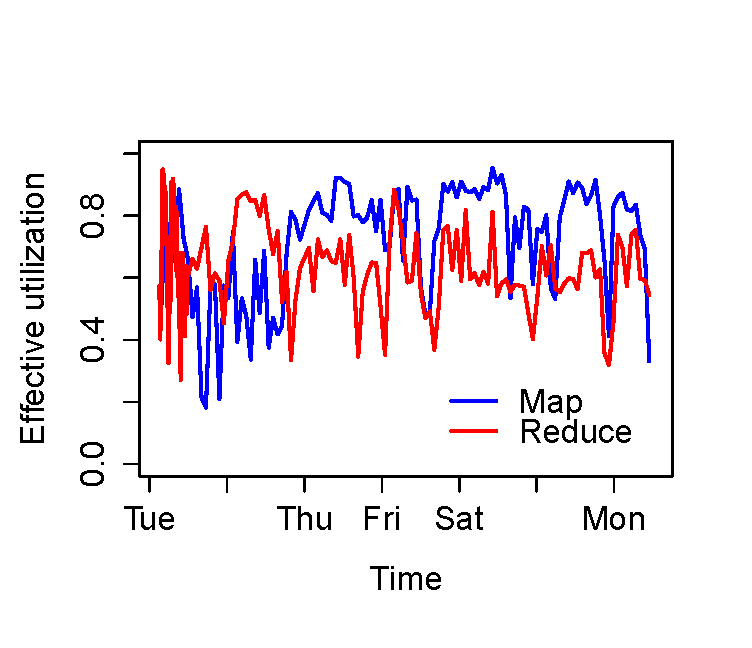
\epsfig{file=eff_util.eps, scale=0.5}
  \caption{Effective map and reduce utilization}
  \label{fig:utilization}
\end{figure}

Figure \ref{fig:utilization} shows $E_m(t)$
and $E_r(t)$ over the week from July 29 to August 4. Alice 
would be surprised by the results in Figure \ref{fig:utilization}:
the average effective utilization for map and reduce is only 72.5\% and
67.3\%, respectively, over this period. Thus, while the cluster 
demand and usage look very high, approximately 30\% of the cluster
resources are being wasted from Alice's perspective. She will 
want to investigate the reasons that are responsible for the 
unexpectedly low effective utilization.
As part of a diagnosis exercise, Alice can generate 
statistics as shown in Table \ref{tab:task-statistics} for 
all the MapReduce jobs run over a one-week period. 

\begin{table}
  \centering
  \caption{Statistics of job and attempt status for a one-week period}
  \begin{tabular}{|c|c|l|} \hline
    Type & Percentage (\%)\\ \hline
    Failed jobs & 3\\ \hline
    Killed jobs & 3.11\\ \hline
    Succeeded jobs & 93.89\\ \hline
    Failed attempts & 0.32\\ \hline
    Killed attempts & 18\\ \hline
    Successful attempts & 81.68\\
    \hline\end{tabular}
    \label{tab:task-statistics}
\end{table}

The table shows that 18.32\% of the 
map and reduce attempts were unsuccessful overall. 
Several factors can lead to unsuccessful attempts. First, 
an attempt will be killed if it is a speculative attempt and the
original attempt for the task has succeeded; or vice versa. Second, 
a MapReduce job can fail due to any number of reasons. Common 
factors include some exception in user code such as a required
file not being found. 

Third, a MapReduce job can be killed by 
the submitting user or by Alice.
A common case seen in practice
is where the job processes heavily-skewed data. Thus, one task
of the job gets hit with a massive amount of data that takes
a very long time to process. Attempts for this task end up causing 
heavy load on the machine where they run, prompting Alice 
to kill the job. A fourth factor is where an attempt gets {\em preempted},
which we will discuss in Section \ref{sec:preemption}. 

\begin{figure}
  \centering
  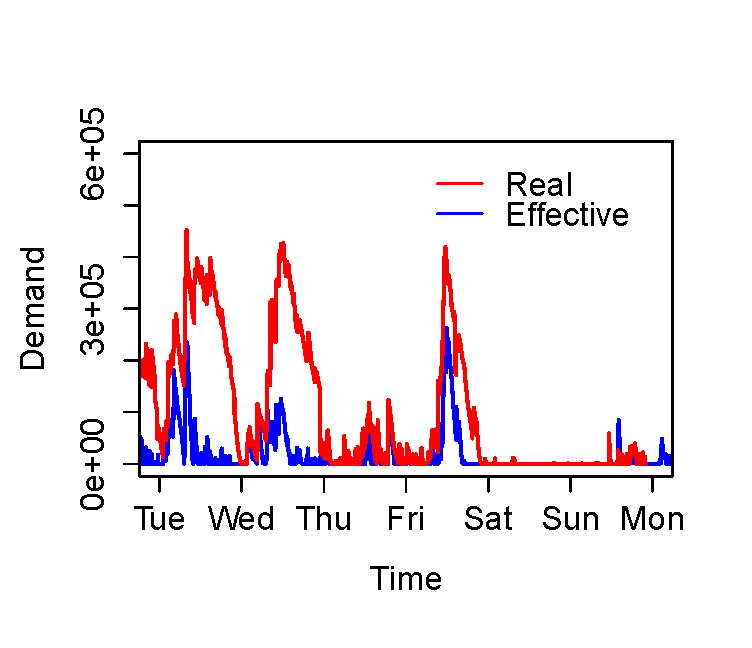
\epsfig{file=analyst_demand.eps,scale=0.5}
  \caption{Map demand of the BI pool}
  \label{fig:BI-demand}
\end{figure}

Figure \ref{fig:BI-demand} shows the map demand in the BI 
pool during the July 29 to August 4 time frame. The ``Real''
plot shows the contributions of this pool 
to the actual map demand, while the ``Effective'' plot
shows the contributions to the effective utilization.
Notice the large gap between the ``Real'' and ``Effective'' plots.
Thus, from Figure \ref{fig:BI-demand}, Alice can conclude that 
the BI pool was one of the contributors to the low effective
utilization seen in the cluster. Applications in the BI pool 
tend to be ad-hoc queries over very large datasets, and 
submitted by users who are not expert users of Hadoop or SQL. 

\eat{
\begin{figure}
  \centering 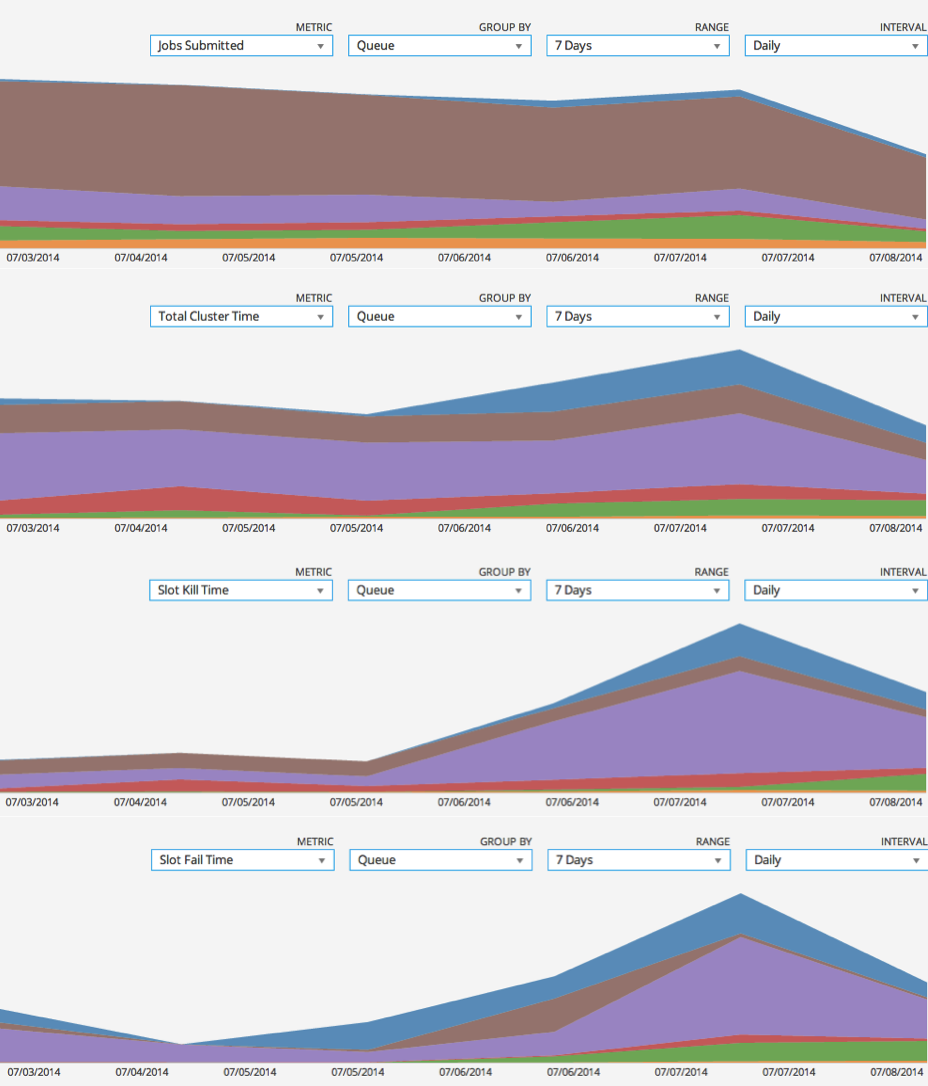
\epsfig{file=CIDR1.eps,scale=0.23}
  \caption{Interactions across pools}
  \label{fig:analyst-Vs-modeling}
\end{figure}
}

\begin{figure}[t!]
        \centering
        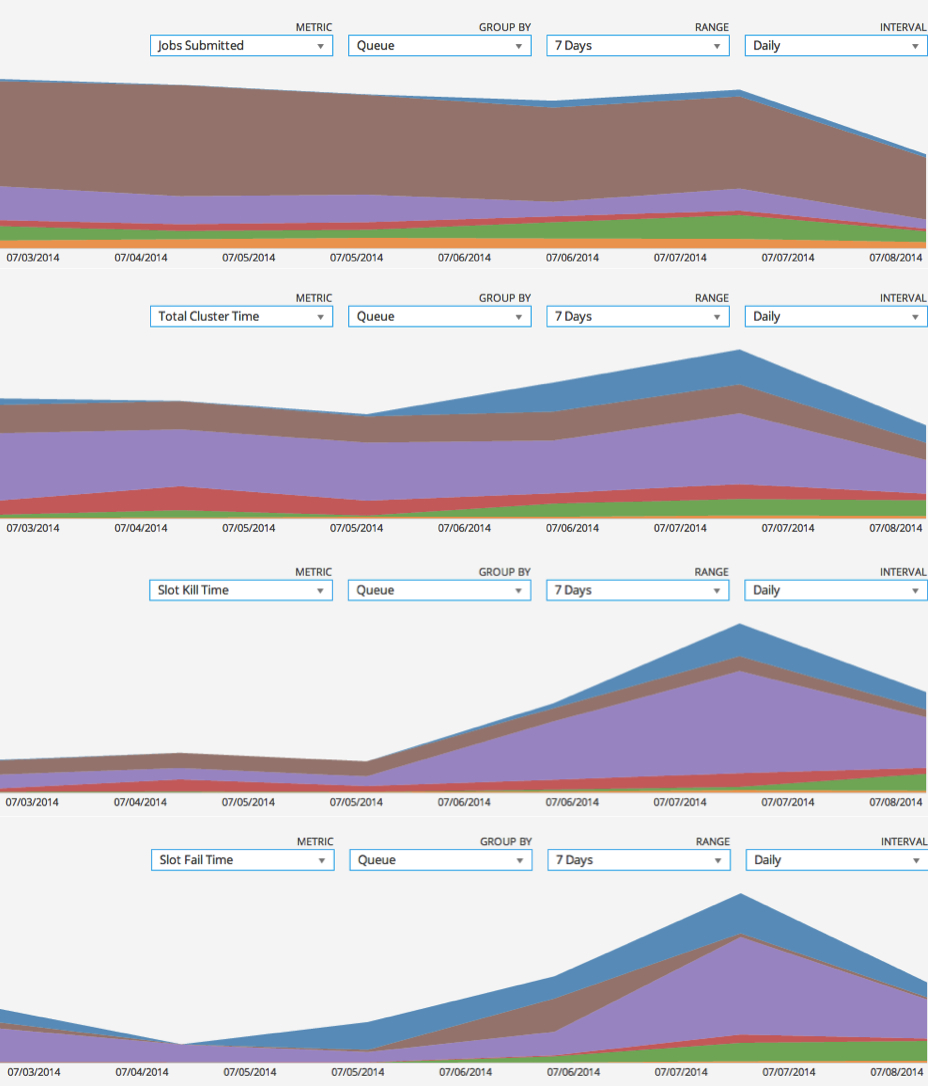
\includegraphics[width=.45\textwidth,height=4.5in]{CIDR2.eps}
        \vspace{-4mm}
        \caption{Interactions across pools}
        \label{fig:analyst-Vs-modeling}
        \vspace{-6mm}
\end{figure}

\subsection {Interactions Across Pools}
Different applications in a pool contend for the same set of resources. 
However, can applications in one pool affect those in another pool?
Figure \ref{fig:analyst-Vs-modeling} shows four performance metrics 
for the pools at Rocket Fuel for a week-long interval. In each
case, the blue, purple, and green areas represents the BI, ETL2, 
and APP2 pools respectively. The following observations can be made 
from Figure \ref{fig:analyst-Vs-modeling} as we go through 
the four performance metrics from top to bottom: 

\squishlist

\item During July 6 and 7, the BI and APP2 pools had a slight increase 
in ``Jobs Submitted'', which is the number of jobs being submitted.
\item During the same dates, the BI pool had a more noticeable 
increase in ``Total Cluster Time'', which is the amount of time 
that applications in each pool spend on the cluster. 
\item The last two performance metrics shown---namely, ``Slot Kill Time"
and ``Slot Fail Time''---denote the amount of time consumed by 
attempts that are eventually unsuccessful. Note how these numbers
went up for the BI and APP2 pools. But much more noticeable is how these
times went up for the ETL2 pool. 

\squishend 

Figure \ref{fig:analyst-Vs-modeling} illustrates the importance of 
answering one common type of question that Alice has to answer:
{\em What will be the impact of an $\alpha$\% increase in the workload in 
the Pool $X$?} This question evolves into a number of other 
questions because the workload can increase in different ways. 
For example, natural growth of data sizes can lead to more attempts
or to more running time per attempt. Or, creation of a new BI application
can lead to an increase in the number of jobs being submitted to 
the BI pool. Avoiding these questions or providing cursory 
answers can have catastrophic consequences on cluster performance. 


\begin{table}
  \centering
  \caption{Configuration parameters for BI pool}
  \begin{tabular}{|c|c|l|} \hline
    Name & Setting \\ \hline
  min\_share\_timeout & 2 hours\\ \hline
                  fair\_share\_timeout & 15 minutes\\ \hline
                  weight & 2.0 \\ \hline
                  map\_min\_share & 2287 slots \\ \hline
                  reduce\_min\_share & 1372 slots \\ \hline
                  sched\_mode & FAIR \\ \hline
    \hline\end{tabular}
    \label{tab:scheduler-config}
\end{table}

\subsection{Controlling the Resource Allocation}
\label{sec:preemption}

Table \ref{tab:scheduler-config} shows the configuration 
parameters per pool that control how Hadoop's Fair
scheduler allocates resources across different pools. 
The ``min share'' and ``weight'' parameters control how the
policy of fair sharing is applied by the 
Fair scheduler. Choosing the settings 
for these parameters that provide the best overall 
workload performance is a challenging task that Alice faces. 
The task becomes even more challenging while 
forecasting growth in the demand for different pools, 
and planning for the resources in advance.

Because of space constraints, we will give only one example, namely, 
regarding the impact of preemptions done by the Fair scheduler.
Premption occurs when the number of slots allocated to a pool goes 
below its {\em minimum share} or half its {\em fair share}
for a certain time interval. During preemption, the 
Fair scheduler will kill the most recently launched attempts in pools 
that have more attempts running than their fair shares. The work 
done by the prempted attempts will be lost when they are killed.

The per-pool ``timeout'' parameters shown in Table \ref{tab:scheduler-config}
determine the time interval mentioned above for which a 
pool will wait before preemptions start. 
Alice usually finds it hard to determine whether to enable preemption and, 
if so, what timeout values to set. On one hand, turning on
preemptions is beneficial for performance-critical pools
to meet SLAs. However, preemption leads to wasted work. 
The best setting depends on SLAs, the workload, and cluster capacity. 

To illustrate the challenges here, Figure \ref{fig:preemption} shows the 
reduce fair share and number of 
running reduce attempts in the ETL2 pool over one day. As can be seen,
the ETL2 pool uses more reduce slots than its reduce fair share over
a five-hour interval. This trend will be surprising to Alice
because preemption of attempts is indeed enabled at Rocket Fuel. 
The reason for the trend seen in Figure \ref{fig:preemption} 
is a combination of the fact that the ETL2 pool has very long-running
reduce tasks and the fact that attempts are preempted
in increasing order of their running time so far. Given 
the characteristics of the workload seen in this pool, 
not enabling preemption could impact severely the chances of 
meeting SLAs in other pools. 

\begin{figure}
  \centering
  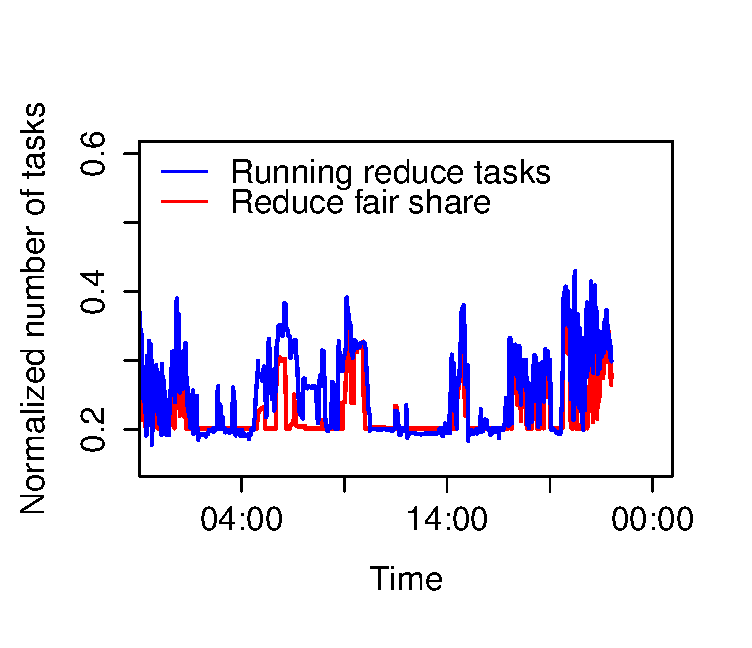
\epsfig{file=long_running_reduces.eps,scale=0.5}
  \caption{Consequences of long-running reduce attempts 
           in the ETL2 pool}
  \label{fig:preemption}
  \vspace{-5mm}
\end{figure}

\subsection{Tuning the Workload in One or More Pools}

Adjusting the per-pool configurations like the ones
in Table \ref{tab:scheduler-config} and Section \ref{sec:preemption}
will enable Alice to control the multi-tenancy. However, 
she would still be playing a {\em zero-sum game} 
because giving more resources to one pool means 
taking away resources from another pool in a contended 
cluster. In this section, we point out five 
different ways in which Alice can make it a 
non-zero-sum game by changing the workload in one or more pools.

\vspace{1mm}
\noindent {\bf Application tuning:}
Tuning queries or jobs in a pool can improve the 
resource usage within the pool as well as free up resources 
for other pools. 

\vspace{1mm}
\noindent {\bf Data layout tuning:}
Tuning data layouts---e.g., changing a table from a text-based 
format to an encoded columnar format---can change the workload
that hits multiple pools. It can be very hard for Alice
to predict the impact of such tuning on the overall multi-tenant
cluster. 

\vspace{1mm}
\noindent {\bf Dependency awareness:}
Analytics workloads can have a number of data-related
dependencies. For example, the input of one job may come 
from another job in a workflow that contains both jobs.
Such dependencies can have significant impact on 
effective utilization. Consider a MapReduce job that 
has long-running map attempts. If reduce attempts for this 
job are started before all map attempts finish, then 
these reduce attempts may not do any useful work for long periods; 
while holding on to slots all the while. We have seen significant 
benefits at Rocket Fuel through tuning that accounts for this behavior. 

\vspace{1mm}
\noindent {\bf Workload shifting:}
As we can see from Figures 
\ref{fig:demand}(a) and \ref{fig:demand}(b), the resource
demand on the cluster has highs and lows. Some of the workloads---e.g., 
those coming from batch applications such as report generation---can
be moved to intervals with low resource demand. 

\vspace{1mm}
\noindent {\bf Admission control:}
Admission control can limit the concurrency level of a pool. 
However, it can be nontrivial for Alice to come up with good
admission control policies given different workload characteristics
per pool as well interactions among pools. We have experienced cases 
where changing the admission control policies for one pool 
led to significant changes in the performance of another pool. 






